\documentclass[a4paper, 12pt]{article}

\usepackage[utf8]{inputenc}
\usepackage[english]{babel}
\usepackage{graphicx}
\usepackage[margin=1in]{geometry}
\usepackage{svg}

\renewcommand{\baselinestretch}{1.15}
\setlength{\parindent}{0pt}
\setlength{\parskip}{0.8em}

\graphicspath{ {../graphs/} }

\begin{document}

\begin{titlepage}
    \centering
    \vspace*{1cm}

    {\Huge \textbf{Comparison of Spatial Partitioning Strategies}}\\[1.5cm]

    {\large Linus Kåreblom}\\[1cm]

    \vfill

    Technical program Academic year 2024/2025\\
    \textbf{School:} Österänggymnasiet\\
    \textbf{Class:} TE3A\\
    \textbf{Supervisor:} Tony Tieu\\

    \vspace{1cm}
    {\today}
\end{titlepage}

\begin{abstract}
    Spatial partitioning is a widely used optimization strategy to efficiently
    optimize objects in space. It can be found in many applications, from
    simulating galaxies to video games.
    Checking collision between objects is an expensive operation that quickly
    becomes a bottleneck as the number of objects grow.
    This paper compares three different strategies, alongside a naive solution.
    The aim is to evaluate the use cases for the different strategies.
    Each strategy was implemented to fit the same interface to make it as fair
    of a comparison as possible.
    The results show how spatial hashing out performs every other method when
    the objects are distributed evenly while quadtrees excel with uneven object
    distribution.
\end{abstract}

\newpage

\tableofcontents
\newpage

\section{Introduction}
When I was developing a small physics engine, I encountered performance issues
during the  collision detection phase. In this phase the program figures out
which objects are close enough to be touching and overlapping. This wouldn't be
an issue in a small simulation with few objects, but I was striving for
something grand running in real time which made every millisecond count. Due to
these constraints I had to find a way to speed things up.

On my optimization journey I encountered the concept of spatial partitioning -
an elegant solution to my problem. Diving deeper I discovered the three
techniques I'll be comparing in this paper, along side the naive solution. The
basic theory of the technique is simply to group objects close to each other to
avoid checking two objects on the opposite side of the world. This drastically
decreases the number of collision checks performed each frame.

As a consequence of this constraint I had to find a way to optimize this phase.
That is what sent me down the rabbit hole of spatial partitioning as an
optimization to do query objects close to each other in space. During my
research I found out about the three strategies I'm comparing in this paper. I'm
doing this paper within the programming course.

\section{Theory}
\subsection{Spatial Partitioning}
Spatial partitioning is an optimization technique used to make programs run
faster. It's often found within physics applications. The theory behind this
technique is to reduce the number of times one object is checked against
another. Suppose we have one hundred objects in our world. The naive way to
check each one of these against the others results in a ten thousand checks.
Since checks are expensive to make, we want to perform as few of them as
possible.

\subsection{Quadtree}
A quadtree is a recursive data structure, meaning it contains pointers to each
objects of the same type as itself. It's in the family of tree data structures.
The data structure is comprised of nodes. Each node has four pointers to other
nodes, could also be referred to as branches or leaves. This strategy works by
inserting points into a leaf until the leaf reaches its capacity, then it splits
into four equally large sub leaves. This subdivision pattern is shown in figure
\ref{fig:quadtree}.

\begin{figure}[ht]
    \includesvg[width=\textwidth]{images/invert-quadtree.svg}
    \caption{Visual representation of a quadtree.}
    \label{fig:quadtree}
\end{figure}

\subsection{The Stack and Heap}
A program uses two different types of memory, the stack and the heap. When the
program starts a fixed amount of bytes are allocated for the program to use,
this is what is called the stack. When the program creates a variable it is
allocated on the stack, which is done by incrementing the stack pointer by the
size of the variable data type. Since a stack allocation is only a single
instruction it is incredibly fast. The heap is much larger than the stack but
slower because you have to request space within it from the operating system.
Allocating is considered to be a slow operation since there's a lot of overhead
introduced.

\subsection{Big O notation}
Big O notation is a notation system to describe the time complexity of an
algorithm. If an algorithm has the time complexity of $O(n)$ then that means
its time complexity grows linearly with the amount of inputs $n$. This could be
deceiving due to a hidden constant within the expression. If $O(n)$ would be
written as a function to describe the actual execution time of the algorithm
then it would look like this $T(n) = C \cdot n$. A $O(n^{2})$ algorithm would
be considered worse than an $O(n)$ one. This assumption is, however, not always
correct. If $n$ is small enough then the $O(n^{2})$ algorithm could run faster
due to the constant being smaller than its $O(n)$ equivalent.

\subsection{Static Grid}
The static grid is built using a simple array. Indexing into the array is an
$O(1)$ operation. The caveat with this approach is you're forced to know how
big the area you want the to partition to be before compiling the program. Both
insertion and querying only requires a simple index into the grid array which
makes this approach super fast.

\subsection{Spatial Hashing Grid}
The spatial hashing grid is built using the same technique as a hash map. The
method I used to write my spatial hashing grid was to allocate an arbitrarily
sized array. When inserting into the structure I first hash the coordinate of
the object, then run a modulo operation on it giving me a number within the
array bounds, and then it is inserted into the cell.

\section{Material and Method}

\subsection{Linux}
Linux is the operating system used to develop the application and write this
paper. The program uses a specific Linux API to acquire the current time as a
UNIX time stamp. The way to do this would differ on other operating systems.

\subsection{Neovim}
Neovim was the editor used to edit the code. It is a modal text editor and not a
full integrated development environment, or IDE as they are called. A plugin
which utilizes the language server protocol was used to provide me with
intellisense and to aid in development by warning me about syntax errors.

\subsection{Git}
Git is a version control system which helps track changes to the project. In
this project it is utilized to keep a time line of the development process and
make sure changes could be synced between devices. The local git repository is
mirrored on GitHub making it accessible from other devices, and the source code
can be read from the browser.

\subsection{CMake}
CMake is a buildsystem, used to generate generate the final executable from the
source code. It aids in compiling and linking the program making cross
compilation and dependency management trivial.

\subsection{C}
C was the program of choice for this project due to its low level control.
Since memory is managed manually in C I could be sure the results would not be
skewed by a garbage collector running in the middle of a benchmark.

\subsection{SDL2}
SDL2 - Simple DirectMedia Layer - is a cross-platform library supplying an easy
API to create a window and render to it. This was crucial when developing since
visualizing the data structures made it easier to spot errors than simply
looking at the code. It also gives a nice visual representation of the program.

\subsection{Python}
Python is an interpreted programming language which was used for making a script
to generate graphs. All the graphs used in this paper was generated from data
collected from a C program, which dumped said data into a JSON file, which was
then read by a Python script using the matplotlib library to generate nice
looking graphs.

\newpage

\section{Results}
This section presents the results of the benchmarking done on the three
strategies - quadtrees, spatial hashing and static grids. The metrics measured
was average runtime: the sum of all operations needed to run the program.
Insertions: how long it took to insert all the objects into the data structure.
Collision testing: total time spent checking objects against each other, which
includes querying. Querying: average time spent retrieving objects from the data
structure. Clearing: how long it takes to reset the data structure making it
ready for rebuilding. Each metric was measured with a range of object count,
labeled as 'box count' in the graphs, from ten to 2500 with an increase of ten
objects between each measurement. At each stage was run 32 times and the results
were averaged to give smoother graphs. Two benchmarks was run, one with an even
distribution of objects and one with an uneven distribution.

\begin{figure}[h]
    \centering
    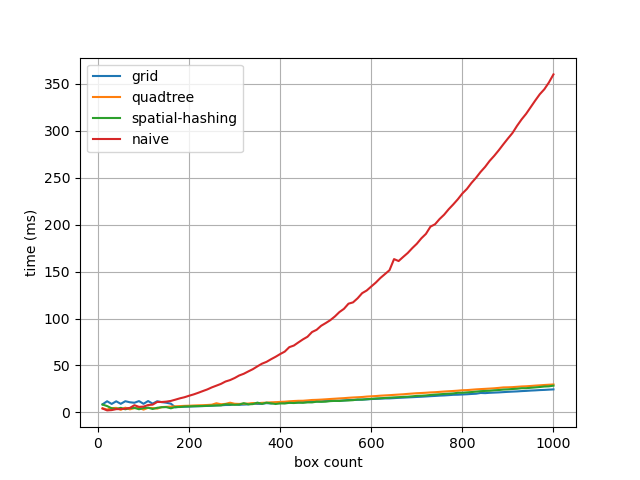
\includegraphics[width=0.5\textwidth]{even-naive.png}
    \caption{Runtime of naive solution and partitioning strategies.}
    \label{fig:naive}
\end{figure}

Figure \ref{fig:naive} shows a drastic difference in runtime between the naive
solution and the optimization strategies. It is hard to evaluate which strategy
performs best due to the stark difference between the naive and the optimized
versions. Due to this discrepancy the naive solution will not be included in the
other graphs presented. This comparison was only run with 1000 objects due to
the time taken per execution.

\subsection{Average Runtime}

\subsubsection{Evenly Distributed Objects}
Figure \ref{fig:even-average} shows the average runtime for the program
using the different strategies with an even object distribution. This includes
all other measuring metrics. The X axis describes the amount of objects being
processed. The Y axis describes how much time was spent in milliseconds
executing the particular step in the program.

\begin{figure}[h]
    \centering
    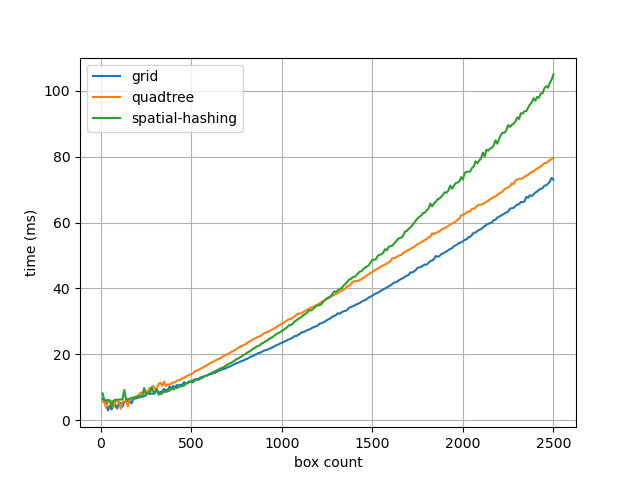
\includegraphics[width=0.5\textwidth]{even-average.png}
    \caption{Average runtime of spatial partitioning strategies with evenly
    distributed objects.}
    \label{fig:even-average}
\end{figure}

\subsubsection{Unevenly Distributed Objects}
Figure \ref{fig:uneven-average} presents the average runtime for the program
using the different strategies with an uneven object distribution. This includes
all other measuring metrics. As the object count increases the spatial hashing
trends towards a $O(n^2)$ runtime complexity.
\begin{figure}[h]
    \centering
    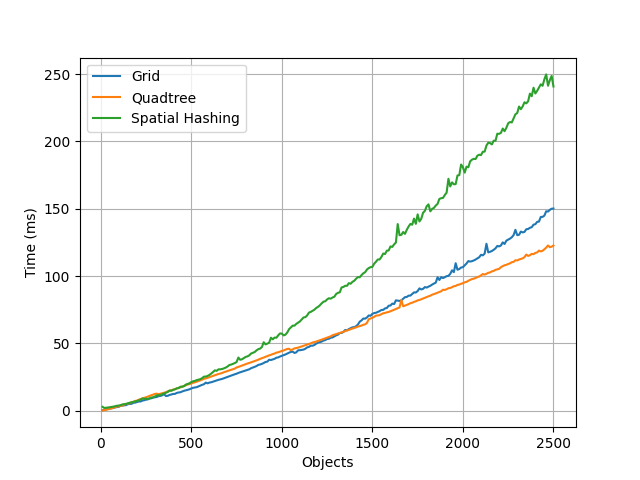
\includegraphics[width=0.5\textwidth]{uneven-average.png}
    \caption{Average runtime of spatial partitioning strategies with unevenly
    distributed objects.}
    \label{fig:uneven-average}
\end{figure}

\subsection{Insertion}

\subsubsection{Evenly Distributed Objects}
The runtime complexity of the insertion algorithms for evenly distributed
objects is shown in figure \ref{fig:even-insert}.
\begin{figure}[h]
    \centering
    \caption{Average insertion time per object with evenly distributed objects.}
    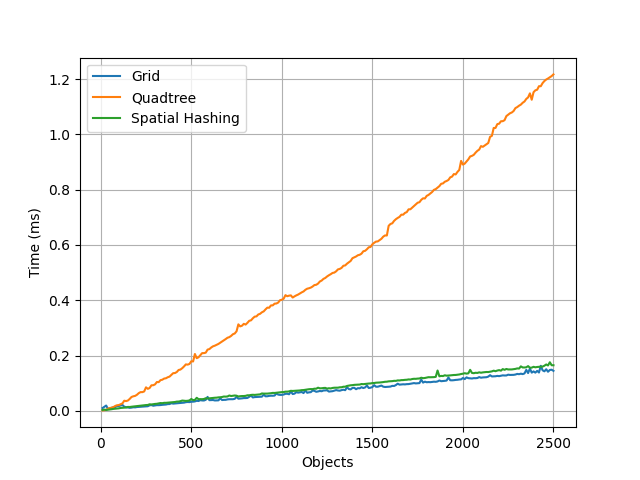
\includegraphics[width=0.5\textwidth]{even-insert.png}
    \label{fig:even-insert}
\end{figure}

\subsubsection{Unevenly Distributed Objects}
The runtime complexity of the insertion algorithms for evenly distributed
objects is shown in figure \ref{fig:uneven-insert}.
\begin{figure}[h]
    \centering
    \caption{Average insertion time per object with unevenly distributed
    objects.}
    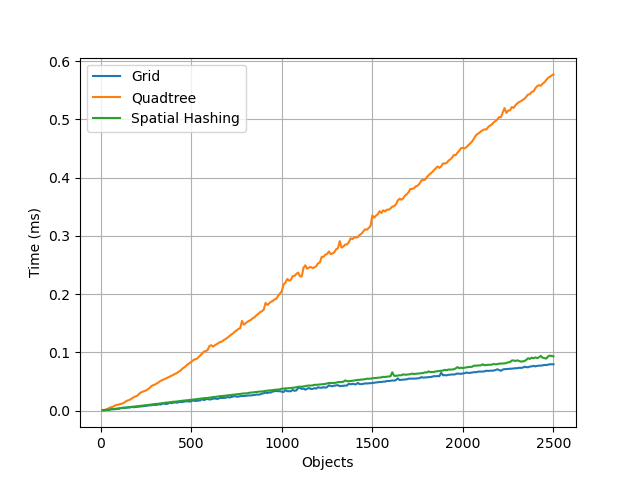
\includegraphics[width=0.5\textwidth]{uneven-insert.png}
    \label{fig:uneven-insert}
\end{figure}

\subsection{Collision}

\subsubsection{Evenly Distributed Objects}
Figure \ref{fig:even-collision} shows the total time spent checking for
colliding objects per iteration with an even distribution. This time also
includes the time taken for querying.
\begin{figure}[h]
    \centering
    \caption{Average collision time for all objects with evenly distributed
    objects.}
    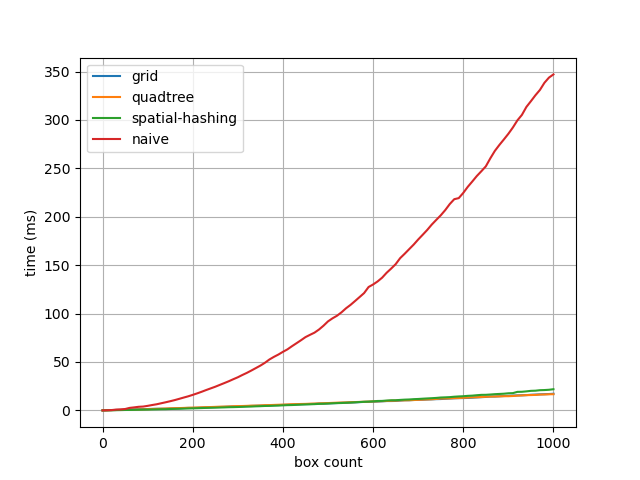
\includegraphics[width=0.5\textwidth]{even-collision.png}
    \label{fig:even-collision}
\end{figure}

\subsubsection{Unevenly Distributed Objects}
Figure \ref{fig:uneven-collision} shows the total time spent checking for
colliding objects per iteration with an uneven distribution. This time also
includes the time taken for querying.
\begin{figure}[h]
    \centering
    \caption{Average collision time for all objects with unevenly distributed
    objects.}
    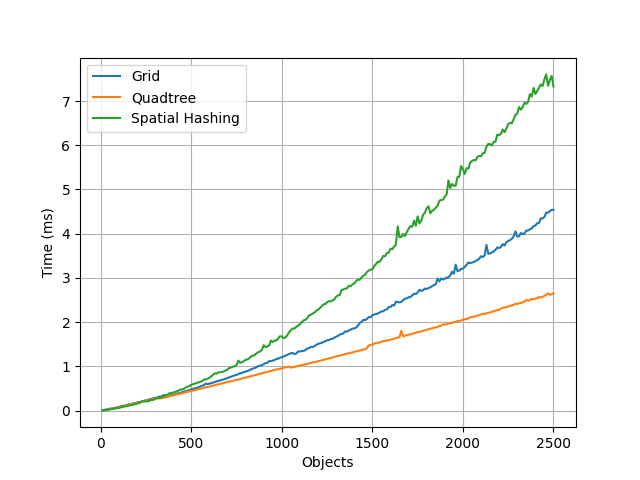
\includegraphics[width=0.5\textwidth]{uneven-collision.png}
    \label{fig:uneven-collision}
\end{figure}

\subsection{Querying}

\subsubsection{Evenly Distributed Objects}
Figure \ref{fig:even-query} represents the average time taken to query the space
per object with an even distribution.
\begin{figure}[h]
    \centering
    \caption{Average query time per object with evenly distributed objects.}
    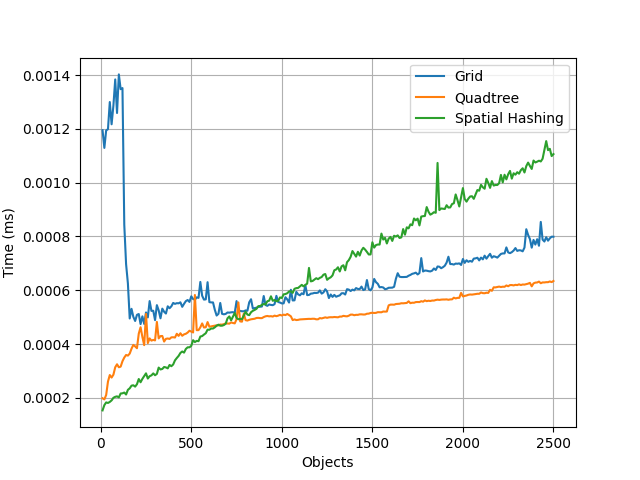
\includegraphics[width=0.5\textwidth]{even-query.png}
    \label{fig:even-query}
\end{figure}

\subsubsection{Unevenly Distributed Objects}
Figure \ref{fig:uneven-query} represents the average time taken to query the space
per object with an uneven distribution.
\begin{figure}[h]
    \centering
    \caption{Average query time per object with unevenly distributed objects.}
    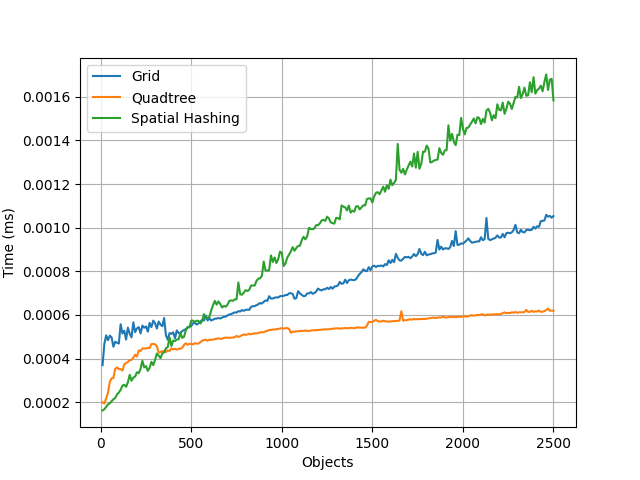
\includegraphics[width=0.5\textwidth]{uneven-query.png}
    \label{fig:uneven-query}
\end{figure}

\end{document}
